% tbp-double on Cu(111)
\begin{wrapfigure}{r}{5cm}\centering
	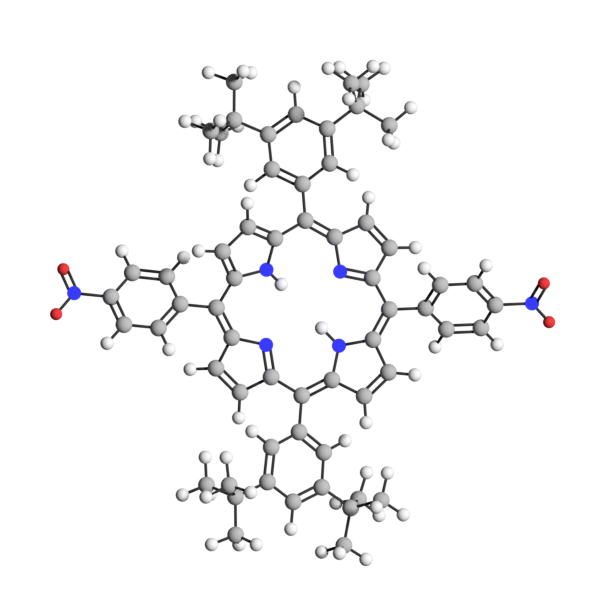
\includegraphics[angle=90, width=5cm]{./images/molecules/max-zoom/TBP-trans-600}
	\caption{}
\end{wrapfigure}

When depositing trans-TBP on Cu(111) at room temperature no long range ordering can be achieved. The molecules arrange rather arbitrarily as can be seen in  \autoref{fig:two-leg-trans-cu111-rt}.

\begin{figure}[h]
 \centering
 \subfigure[]{
 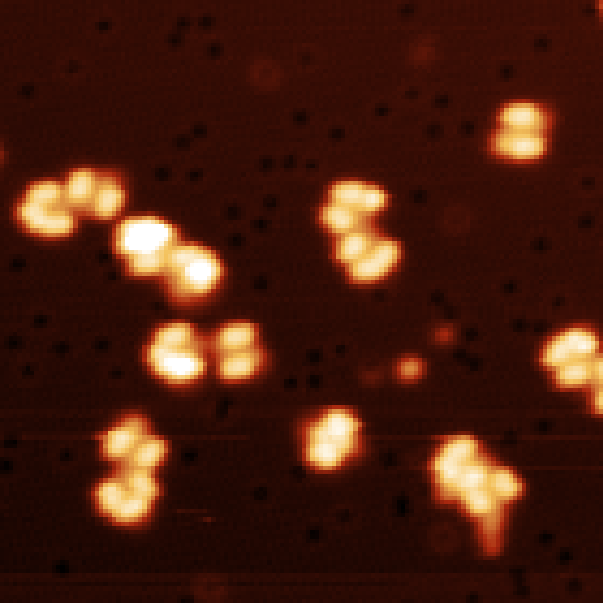
\includegraphics[width=0.3\textwidth]{./images/F160425-172349-40nm}
 %IMAGE SCANNED COARSE!!
 \label{fig:two-leg-trans-cu111-rt}
 }
 \subfigure[New preparation adsorbed at \SI{70}{\celsius}]{
 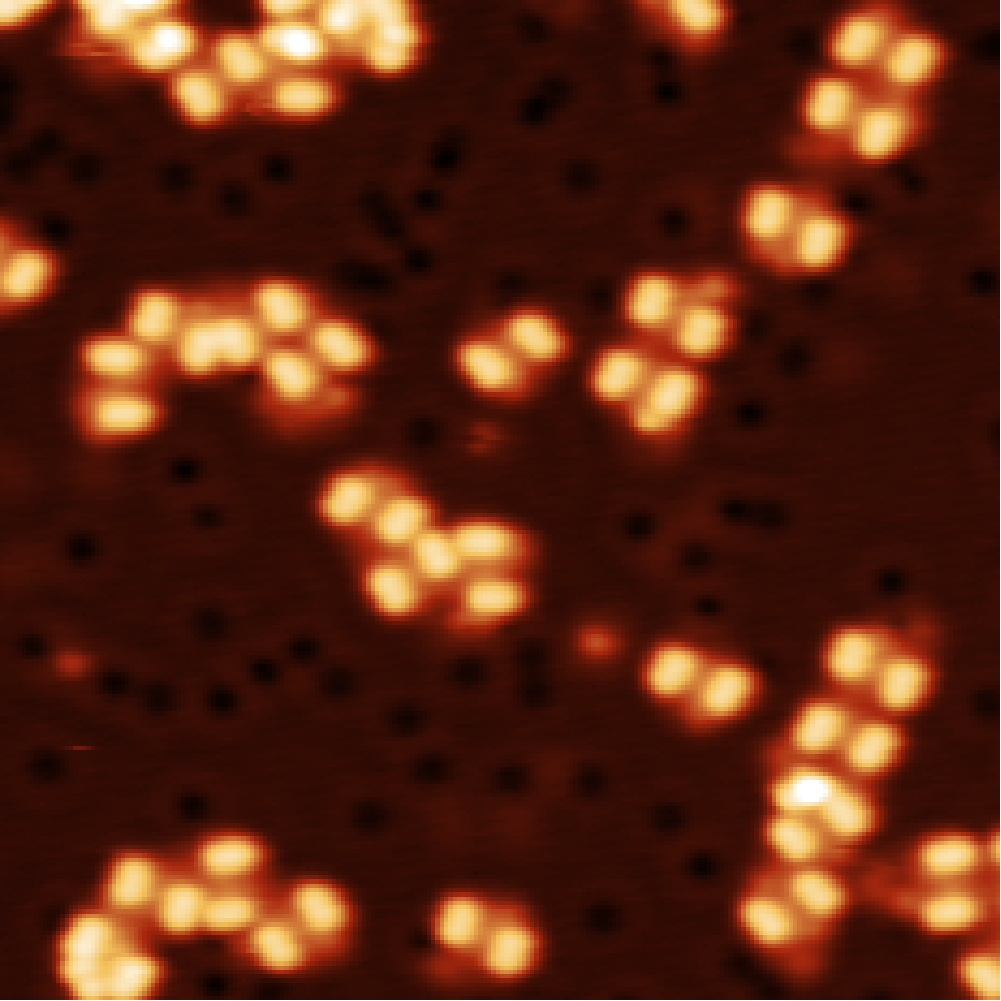
\includegraphics[width=0.3\textwidth]{./images/F160427-121720-40nm}
 \label{fig:two-leg-trans-cu111-70c} 
 %IMAGE SCANNED COARSE!!
 }
 \subfigure[... and heated for \SI{10}{\minute} to \SI{170}{\celsius}]{
 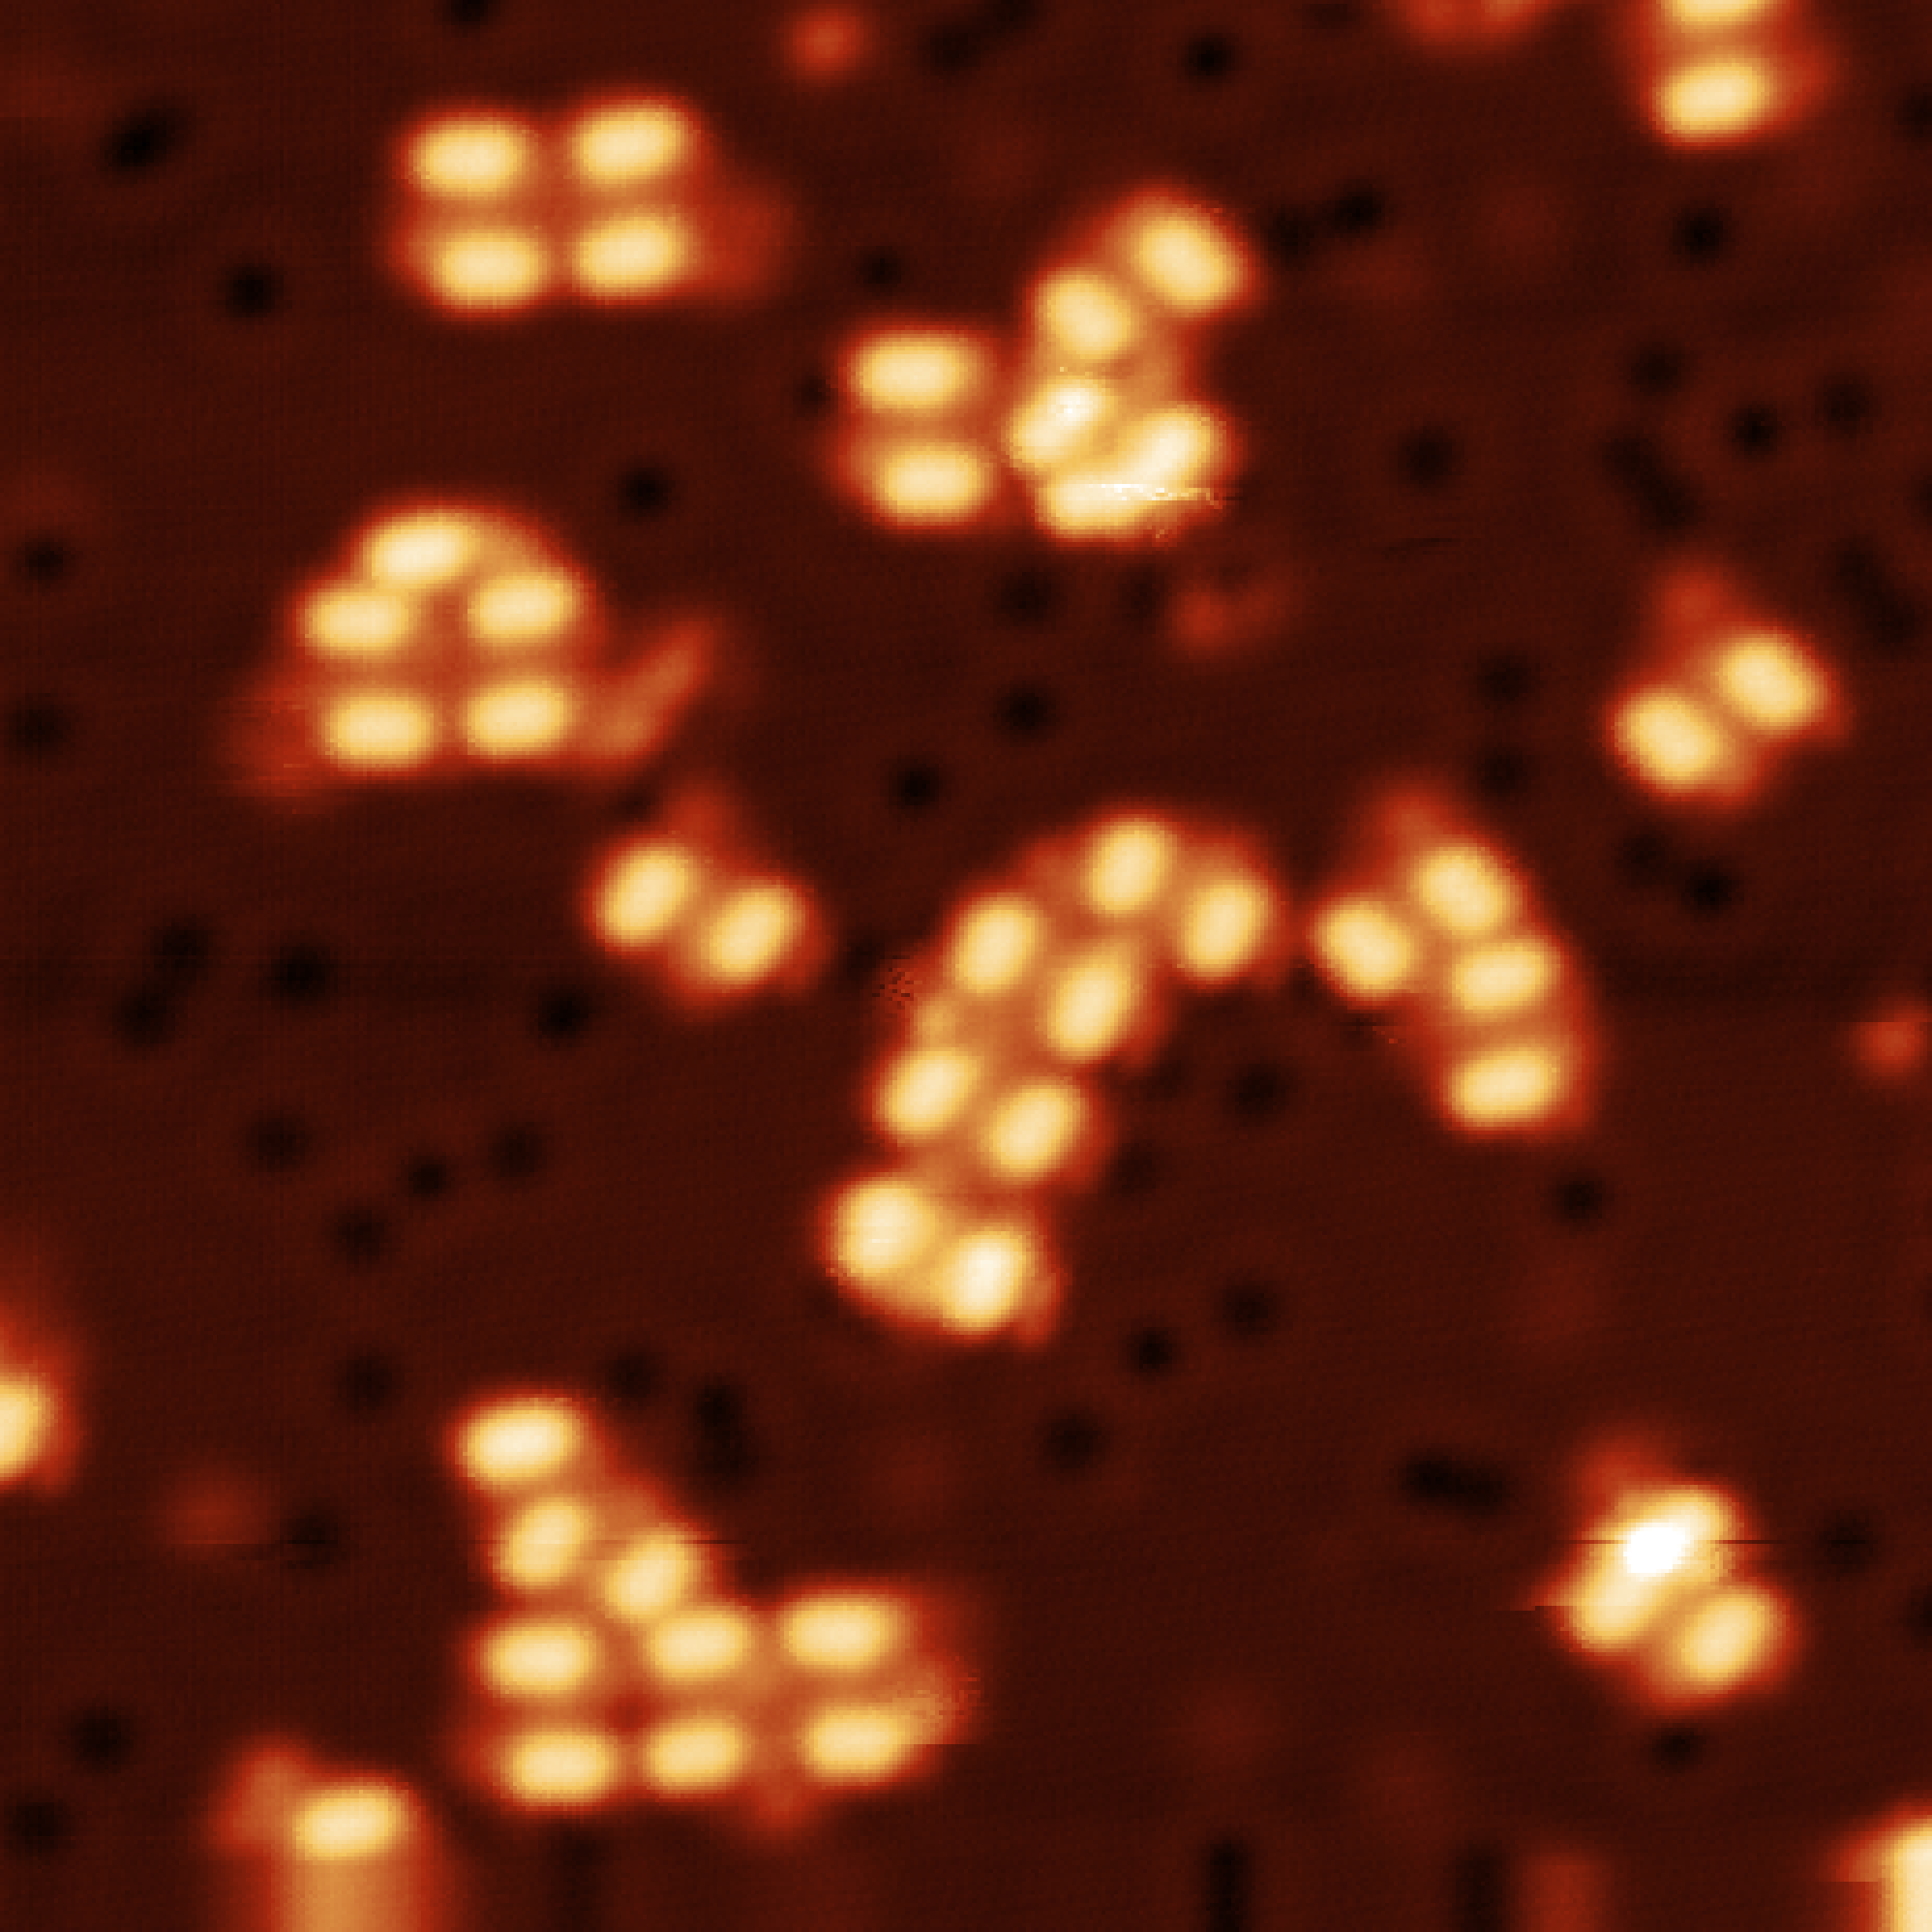
\includegraphics[width=0.3\textwidth]{./images/F160427-142006-40nm}
 \label{fig:two-leg-trans-cu111-170c}
  %IMAGE SCANNED COARSE!!
 }
\caption{Molecules adsorbed on Cu(111) at RT and subsequently annealed to different temperatures. \subref{fig:two-leg-trans-cu111-rt} Adsorption at room temperature did not show extended long range order. \subref{fig:two-leg-trans-cu111-70c}  Adsorption at \SI{70}{\celsius} and \subref{fig:two-leg-trans-cu111-170c} annealing to \SI{170}{\celsius} for \SI{10}{\minute} improves the chain length slightly. All images are \SI{40}{\nano \meter} wide. Scan parameters: \subref{fig:two-leg-trans-cu111-rt} $U_b=\SI{1.2}{\volt}, I_t=\SI{0.041}{\nano \ampere}$, \subref{fig:two-leg-trans-cu111-70c} $U_b=\SI{0.5}{\volt}, I_t=\SI{0.038}{\nano \ampere}$, \subref{fig:two-leg-trans-cu111-170c} $U_b=\SI{0.522}{\volt}, I_t=\SI{0.021}{\nano \ampere}$}
\label{fig:two-leg-trans-cu111}
%ALL OF THE IMAGES SCANNED COARSE!!
\end{figure}

The molecules tend to connect in a defined angle to its next neighbor, forming different binding motifs. These are predominantly different kind of chain formation (see figure \ref{fig:two-leg-trans-cu111-motifs}).
\begin{itemize}
 \item The molecules are ordered such that they form a straight chain (\autoref{trans-nitro-on-cu111-70-straight-chain}).
 \item The molecules arrange in chains, but each molecule has an offset of about a half of its width to the next neighbor or the molecules attach in chains, but show a kink. \autoref{trans-nitro-on-cu111-70-shifted-chain}
\end{itemize}

\begin{figure}[h]
 \centering
 \subfigure[Straight chain]{
 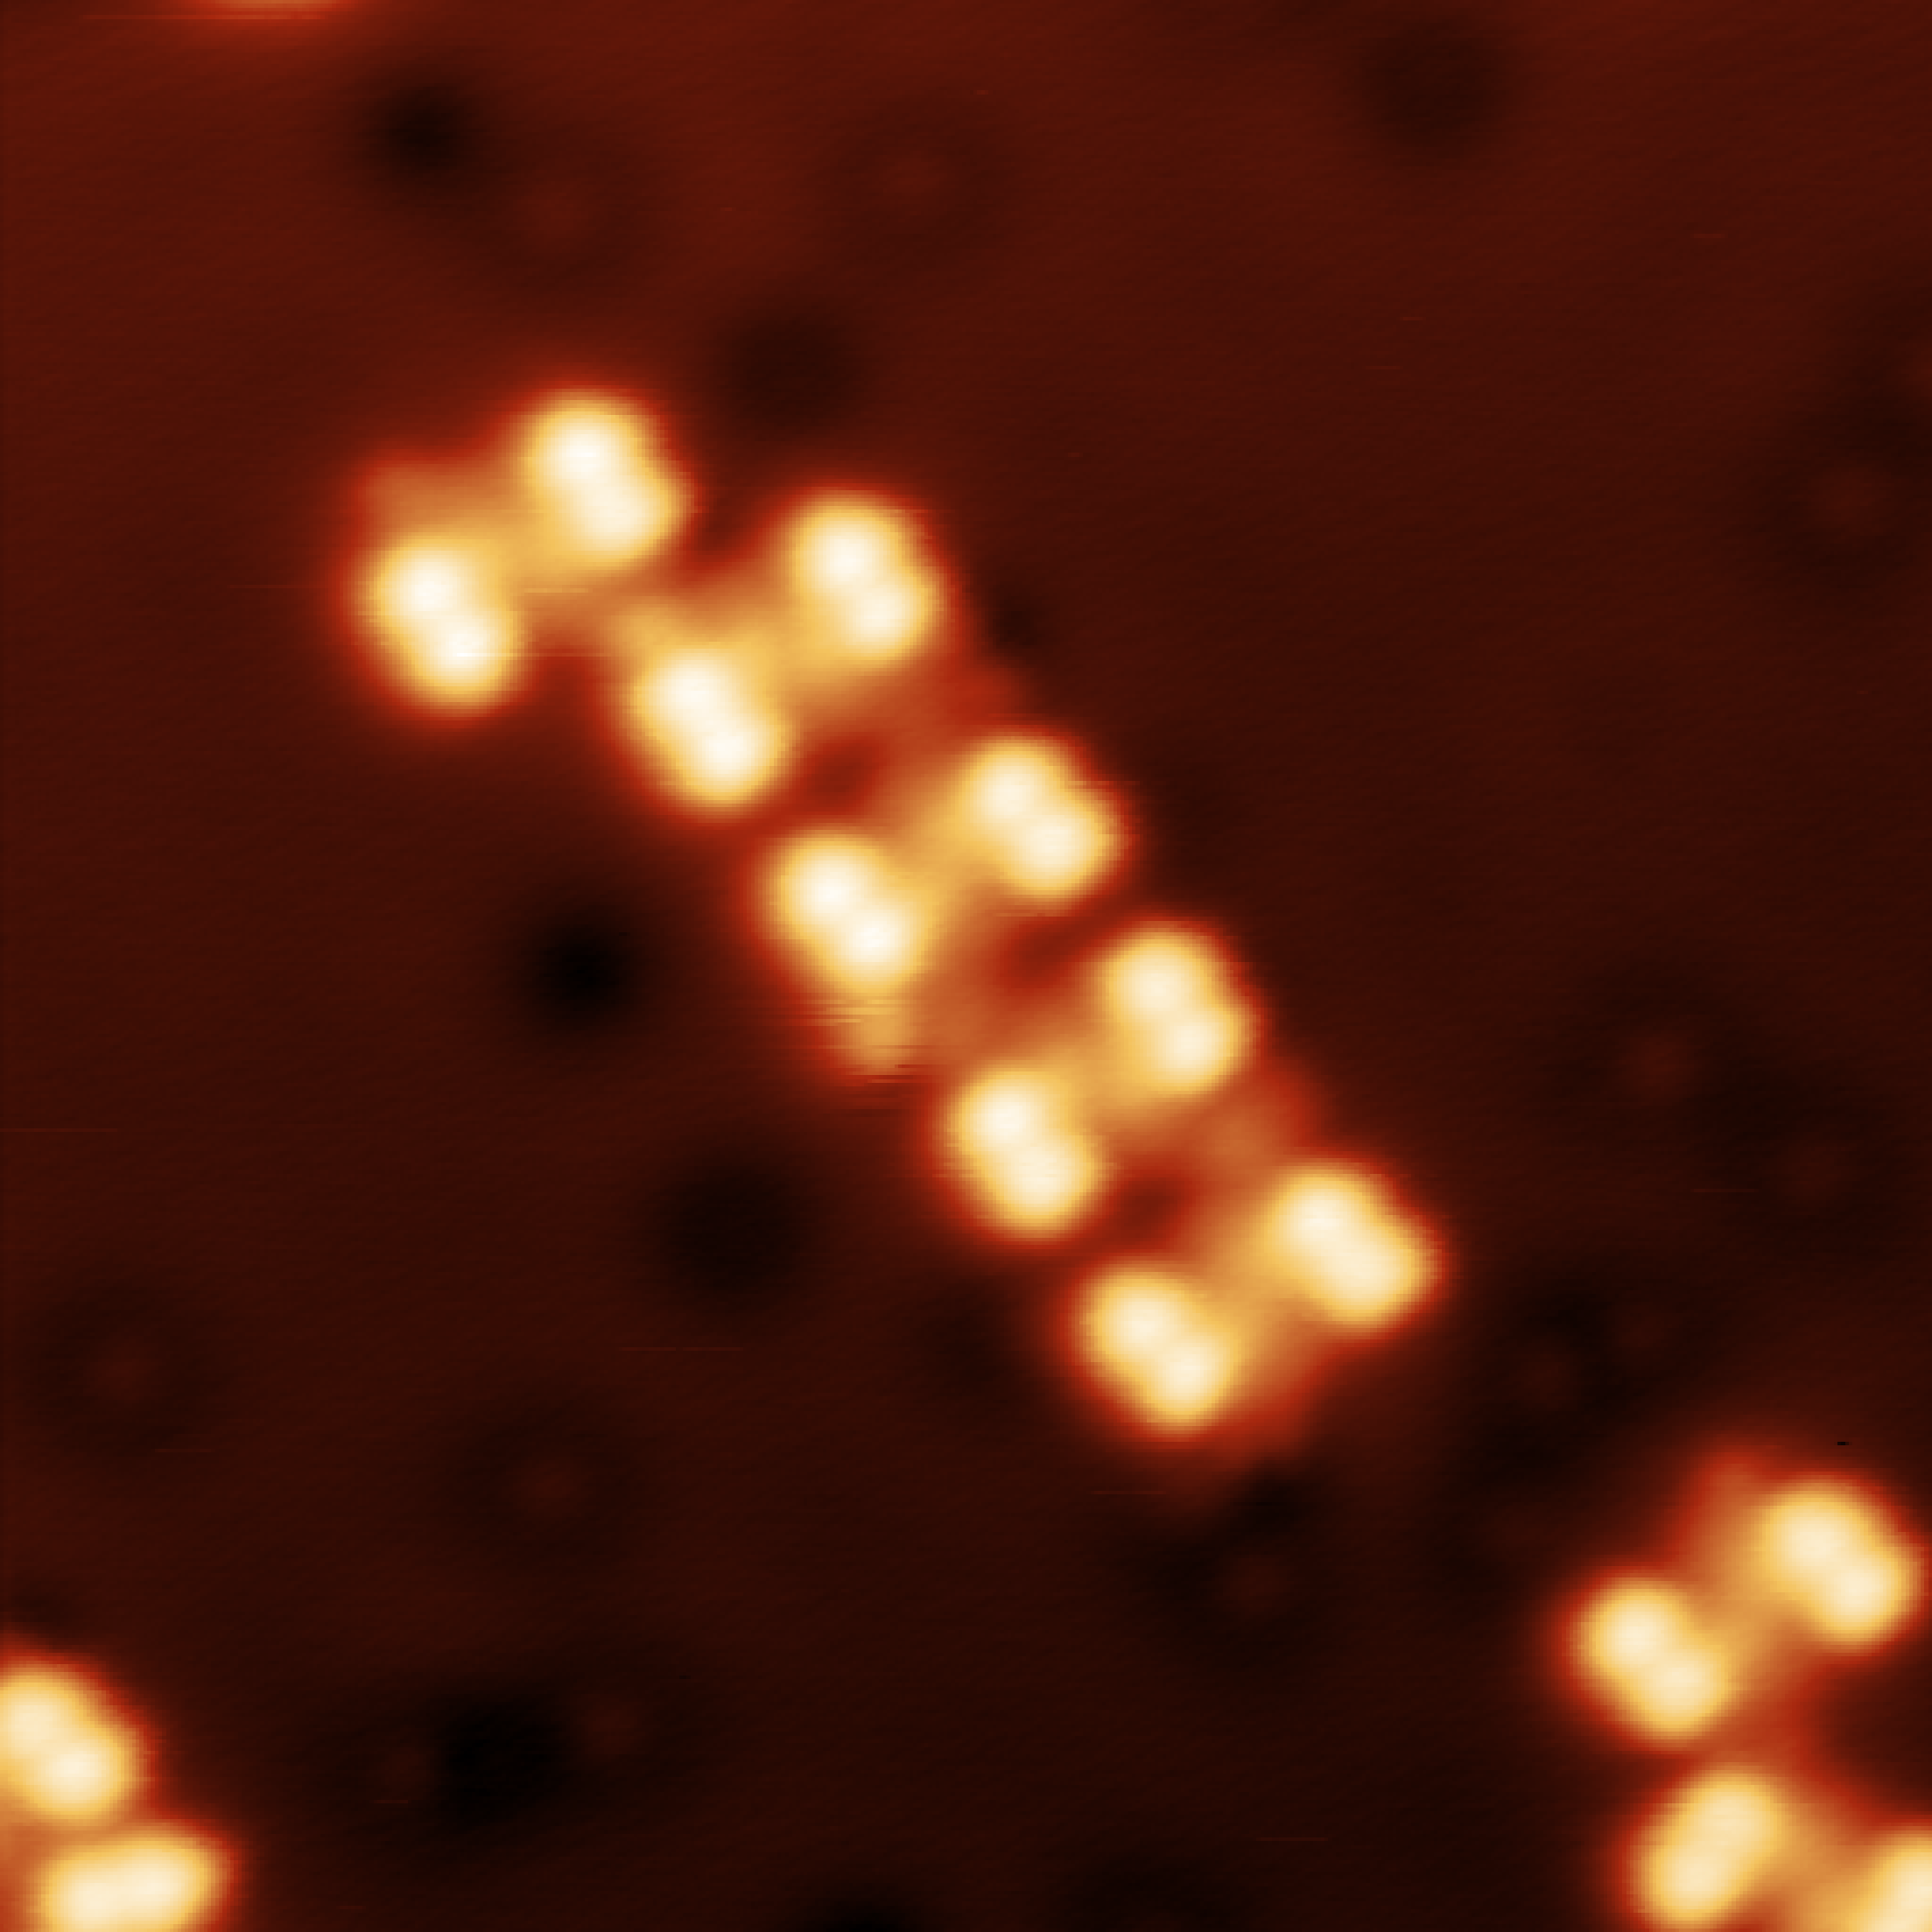
\includegraphics[width=0.45\textwidth]{./images/F160427-154618-R}
\label{trans-nitro-on-cu111-70-straight-chain}} \qquad
 \subfigure[Shited offset chain, interrupted by a kink]{
 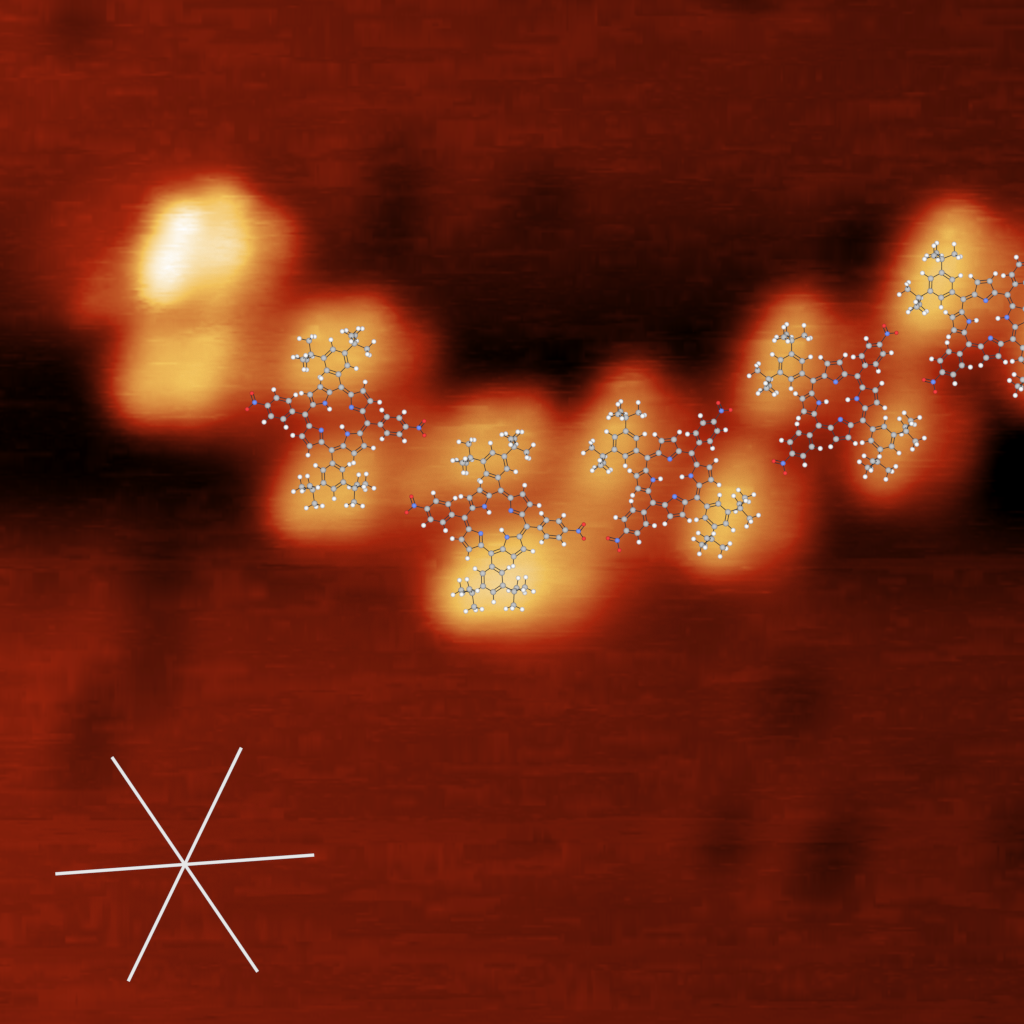
\includegraphics[width=0.45\textwidth]{./images/trans-nitro-on-cu111-120.png}
\label{trans-nitro-on-cu111-70-shifted-chain}}
\caption{All motifs exist at every temperature, although the chain length increases with temperature. It also looks like the chains are getting more offset- and kinked-like chains than at lower temperatures.}
\label{fig:two-leg-trans-cu111-motifs}
\end{figure}

\begin{figure}[h]
	\centering
	\begin{minipage}{0.45\textwidth}
		\subfigure[]{
			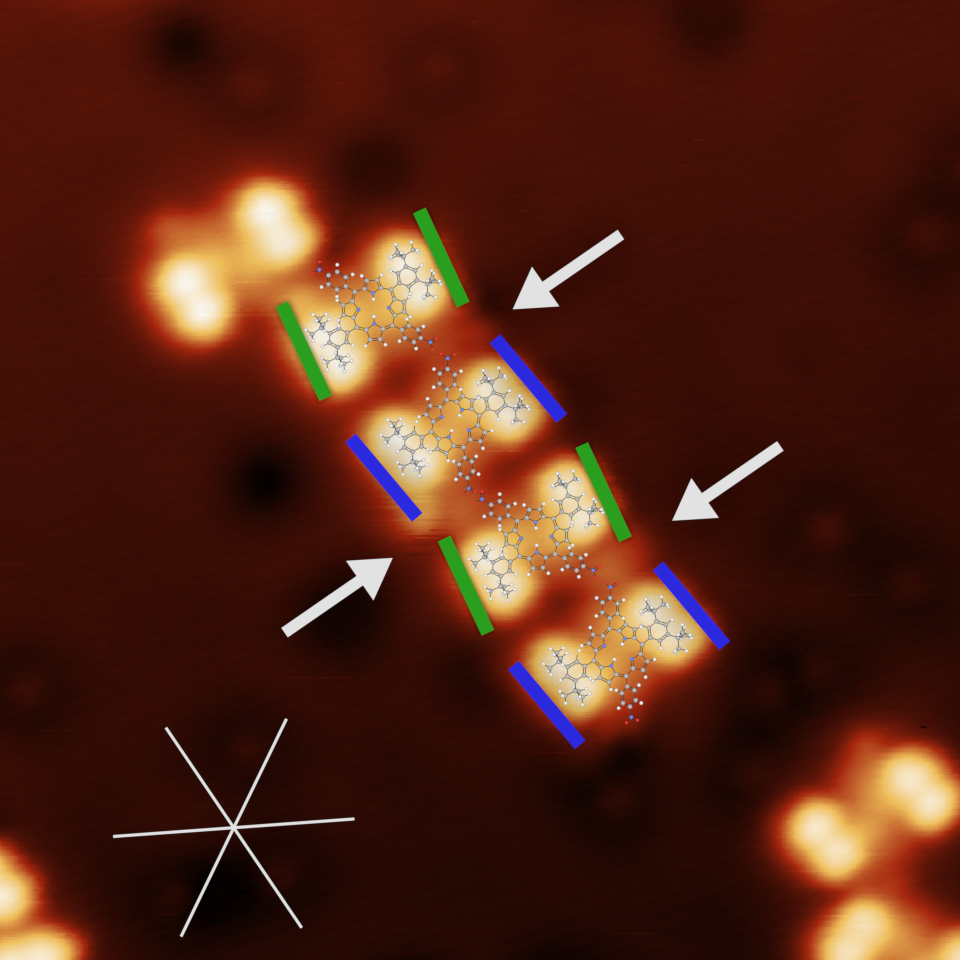
\includegraphics[width=\textwidth]{./images/F160427-154618-R-model}
			\label{trans-nitro-on-cu111-70-straight-chain-II}
		}
	\end{minipage}
	\begin{minipage}{0.45\textwidth}
		\subfigure[]{
			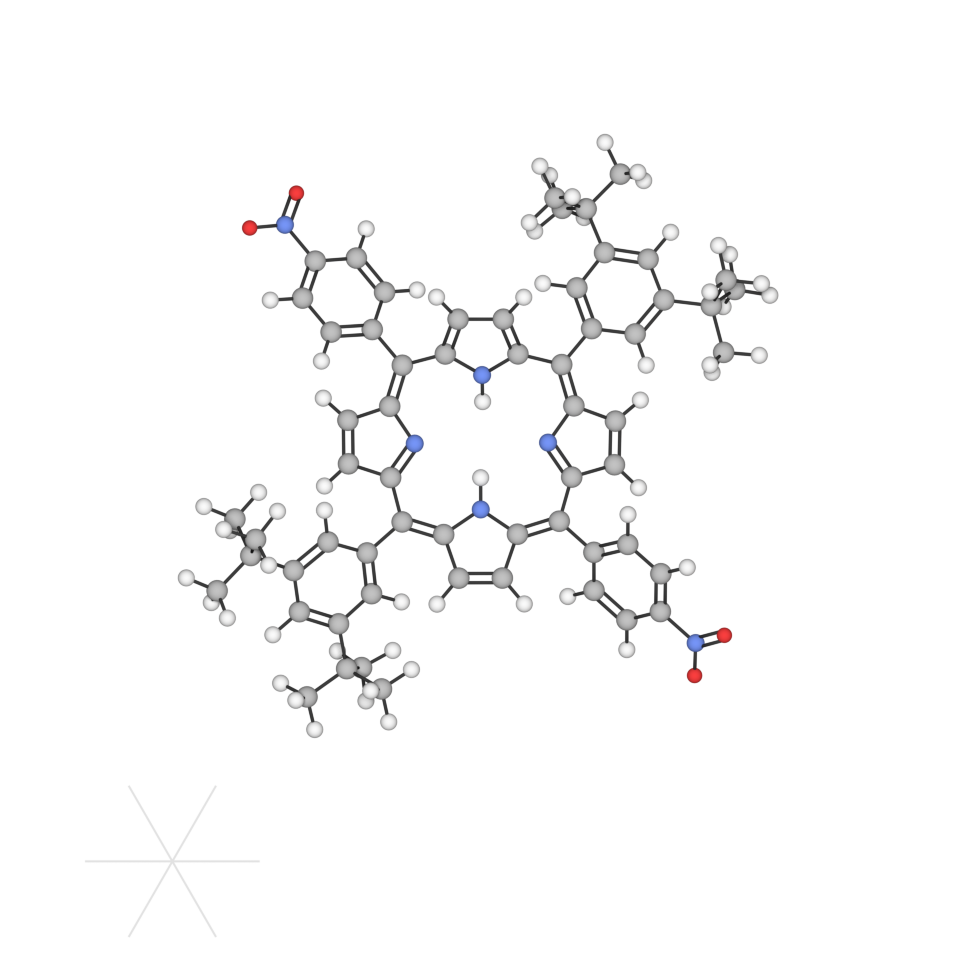
\includegraphics[width=0.45\textwidth]{./images/F160427-154618-R-gas-phase-top}
			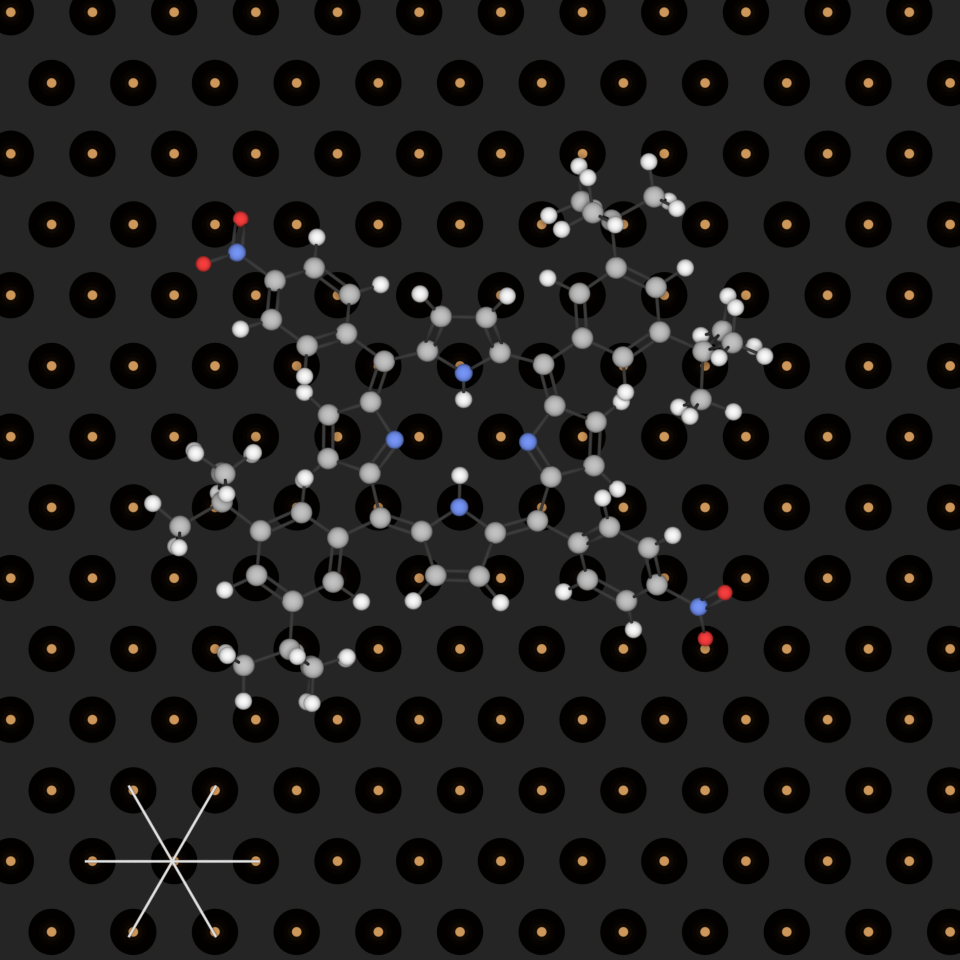
\includegraphics[width=0.45\textwidth]{./images/F160427-154618-R-cu111-top}
			\label{trans-nitro-on-cu111-70-shifted-chain-top-views}
		}
		\subfigure[]{
			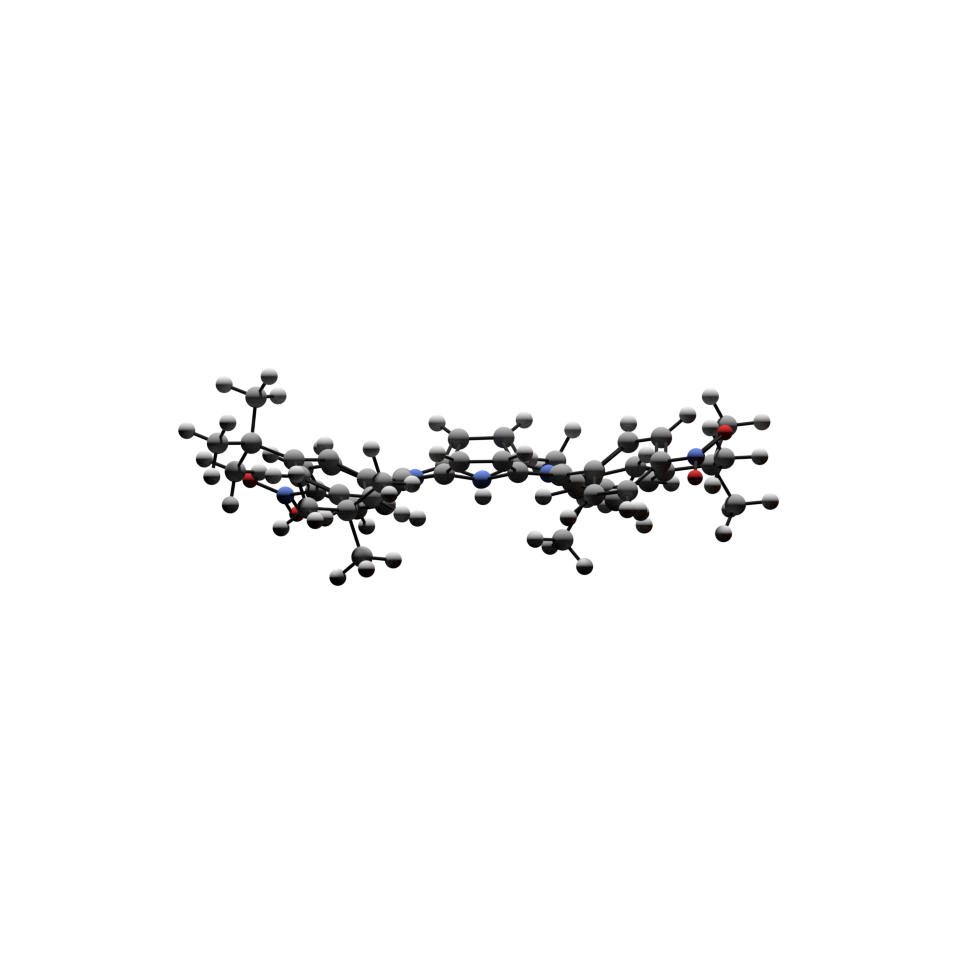
\includegraphics[width=0.45\textwidth]{./images/F160427-154618-R-gas-phase-side}
			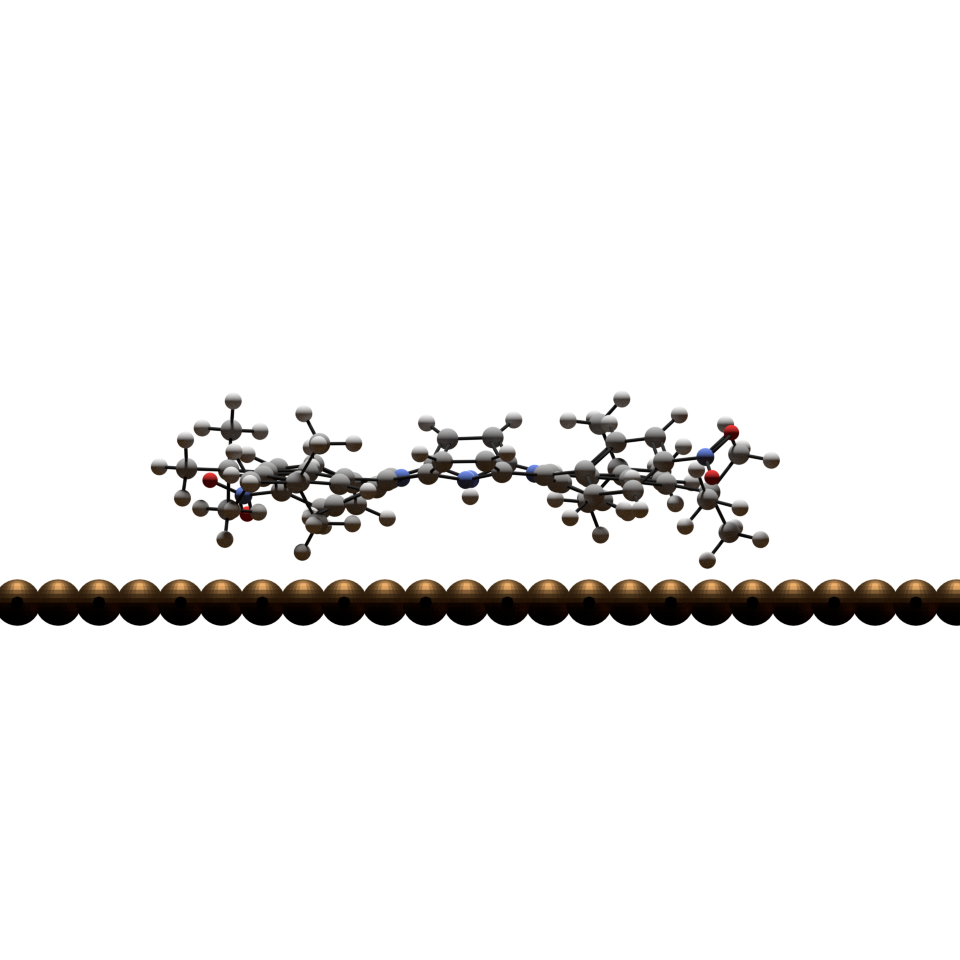
\includegraphics[width=0.45\textwidth]{./images/F160427-154618-R-cu111-side}
			\label{trans-nitro-on-cu111-70-shifted-chain-side-views}
		}
	\end{minipage}
	\caption{Straight chain binding motif on Cu(111). \subref{trans-nitro-on-cu111-70-straight-chain-II} shows an STM image together with the dense packed row indication of the substrate (white lines). Colored bars indicate the rotation of the di-tert-butyl-groups. Arrows point at places where ad-atoms are considred.
		\subref{trans-nitro-on-cu111-70-shifted-chain-top-views} Top views (\SI{6}{\nano \meter} wide) showing the molecules geometry in gas-phase (left) and after adsorption and assembly (right). Although the exact adsorption site is not known, it is considered to by on a bridge site as for 2H-P/Cu(111).
		\subref{trans-nitro-on-cu111-70-shifted-chain-side-views} Side views of above shown configurations.
	}
	\label{fig:two-leg-trans-cu111-motifs-1}
\end{figure}

During modeling \autoref{fig:two-leg-trans-cu111-motifs-1} several points became clear. 
\begin{itemize}
	\item First consider the even apparent height of the di-tert-butyl groups. It indicates that both groups in a legs have comparable heights and it is likely that the phenyl ring bearing these groups is rotated for an even alignment of the tert-butyl groups with regard to the substrate level.
	\item Orientation of di-tert-butyl phenyl groups is the same within a single molecule but alternates (by $\approx \SI{10}{\degree}$) in neighboring molecules in a chain. This is indicated by blue and green lines in \autoref{trans-nitro-on-cu111-70-straight-chain}, each representing a common orientation.
	\item Second the minor contrast variations in the central porphine core change as the orientation of the di-tert-butyl-groups. Free base porphine core is likely to adsorb with its axis  - formed by opposing nitrogens in the core - aligned parallel to the dense packed crystal direction\cite{rojas_surface_2012}. In the present case, the molecule is lifted from the substrate by the bulky di-tert-butyl groups. Hence the porphine core interaction with the crystal substrate is considerable lower than in the 2H-P case. Still, every second molecule has the same orientation, while neighboring molecules are rotated by \SI{30}{\degree}.
	\item The gap between di-tert-butyl-phenyl groups of neighboring molecules is larger on one side of the chain than on the other and shows a larger apparent height (white arrows in \autoref{trans-nitro-on-cu111-70-straight-chain}). Although identification of surface ad-atoms is not straightforward with an STM, they are believed to originate from the copper surface.
\end{itemize} 
The best fitting model consists of molecules with a center-center distance of \SI{1.9 \pm 0.1}{\nano \meter}

Having a closer look to the nitro groups, one recognizes a close proximity of these to each other. Also note the light protrusions in between two adjacent molecules' butyl groups (adatom?). If the legs are rotated by just \SI{15}{\degree}, the nitro groups would point to these protrusions. This rotation costs not much energy and is about \SI{25}{\kilo\J/per\mol} \textcolor{red}{\textbf{(( please cite something, value is for rotated phenyl ring at a porphine core I guess ))}}. Considering these protrusions as Cu-ad atoms (already occurred in chapter \ref{chapter:TPCN-adatoms} as protrusions in between TPCN chains which may change their position in discrete position in the molecule.) This Cu-ad atom may direct the binding of the nitro groups towards it, making them bend outwards. The position of the cooper atom itself may rely on its registry to the substrate - preferring a threefold coordination site as known for copper  \textcolor{red}{\textbf{(( citation ))}}.

The second motif is a chain motif, too. Orientation of molecular axis and dense packed substrate atom rows are the same and again the di-tert-butyl groups orient along them. The difference is a lateral offset between the molecules to shift each of them by half a molecules width. The center-center distances are \SI{1.9 \pm 0.1}{\nano \meter}. It is harder to quantify a possible orientation of the nitro-phenyl groups, since as well straight as well as bended configurations match the assembly. In this binding motif, stable connections between molecules are most likely due to nitro-phenyl groups pointing to di-tert-butyl groups and therefor stabilizing the assembly.

